\documentclass{article}
\usepackage{amssymb}
\usepackage{setspace}
\usepackage{csquotes}
\usepackage{graphicx}
\usepackage{float}
\usepackage{blindtext}
\graphicspath{ {./images/} }
\usepackage[font={small,it}]{caption}

\doublespacing
\begin{document}

\title{%
  Atari Pong AI via Reinforcement Learning \\
  \large Ghost in the Machine Paper \#1}
\author{Ozaner Hansha}
\date{February 20, 2019}
\maketitle

\abstract{This paper has two main goals: 1) To explain, in broad terms, the construction of an artificial intelligence trained to play Atari Pong via reinforcement learning and 2) to use that AI as a vehicle in exploring how modern advances in artificial neural networks and deep learning may change our perception of what constitutes `thinking' in a computer.}

\section{The Problem}
\subsection{Hard-coded vs. Learned}
Our goal is to create a learning agent, a program, that can defeat an opposing hard-coded agent at Atari Pong. Here `hard-coded' refers to a program that does not make use of machine learning algorithms and techniques. This means that the AI is the product of a human programmer analyzing and engineering an algorithm specialized to playing Atari Pong. This is opposed to our AI, which will be using a general purpose \textit{learning algorithm} and gradually get better at playing pong as it plays more games. At least that's the hope.

This key difference between the two AIs is the object of this paper. Indeed, a pong playing AI is not very impressive in this day and age, but a AI that \textit{learned} to play pong? Programs such as these, which have only come into existence relatively recently, have far more interesting implications which we will touch upon later in the paper.
\subsection{The Game}
The game environment is simulated via OpenAI's \texttt{gym} python package, and is one of many Atari games included in it. This fact isn't too important to our purposes, however, as Pong is a relatively simple game with little variation between versions.

Each training match between these two AIs is called an \textit{episode}, and each episode goes on until one player reaches 20 points. As we'll see below, whenever the AI loses a round it is given negative feedback associated with its actions (i.e. `punished') and positive feedback when it wins (i.e. `rewarded'). It is from this simple incentive mechanism that reinforcement learning, a type of machine learning which we are about to explicate, gets its name.



\section{The Algorithm}
Reinforcement learning is an umbrella term for machine learning techniques that model how \textit{agents} can best take \textit{actions} that affect some \textit{environment} that, hopefully, maximize some quantified \textit{reward}. In our case, the Pong AI is the agent, the actions it can take are moving the paddle up and down, the environment it affects is the board, ball, and other player, and the reward is getting the ball past the other paddle (not the score because, as we'll see, its not that important to the AI in the long run).

\subsection{The Input}
Note that the only input we are allowing ourselves to use is the raw pixel data from the game's screen. This way we can't protest that the AI has an unfair advantage when compared to a human, disregarding the fact that our AI can process information billions of times faster than a human and was mathematically constructed to win at Pong...

In any case, at every time step our AI's input is the current frame of the game: a single $210\times160\times 3$ three dimensional array. The first two dimensions correspond to the length and width of the image while the third correspond to the 3 color channels red, green and blue.

\begin{figure}[h]
\centering
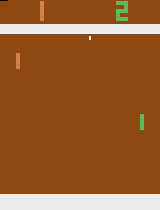
\includegraphics{frame}
\caption*{A frame of Pong in its raw, image form.}
\end{figure}

You'll notice, however, that much of this pixel data is useless to our AI's purpose. For example, the color doesn't help our AI perform any better, and so we may as well remove that input before feeding it to the network. This instantly reduces the dimensionality of our input by a factor of 3. We can go even further by trimming the image of its corners, including the score. It's not like the behavior of the opponent AI will change depending on who has the lead. Maybe it would be useful information if the AI was pitted against a human player whose behavior \textit{would} vary with the score counter, but not in this case. Trimmed and grayscaled, our preprocessed input looks something like this:

\begin{figure}[h]
\centering
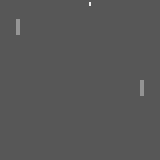
\includegraphics{frame_pp}
\caption*{A more drab, yet more information dense, preprocessed frame of Pong.}
\end{figure}

\vspace{-.1cm}

\subsection{The Artificial Neural Network}
The function which will take in this pruned input image and output whether or not we should move our paddle up or down will be an artificial neural network or ANN. The general structure of an ANN is as follows:

\vspace{-.4cm}
\begin{figure}[H]
\centering
\hspace*{-2cm}
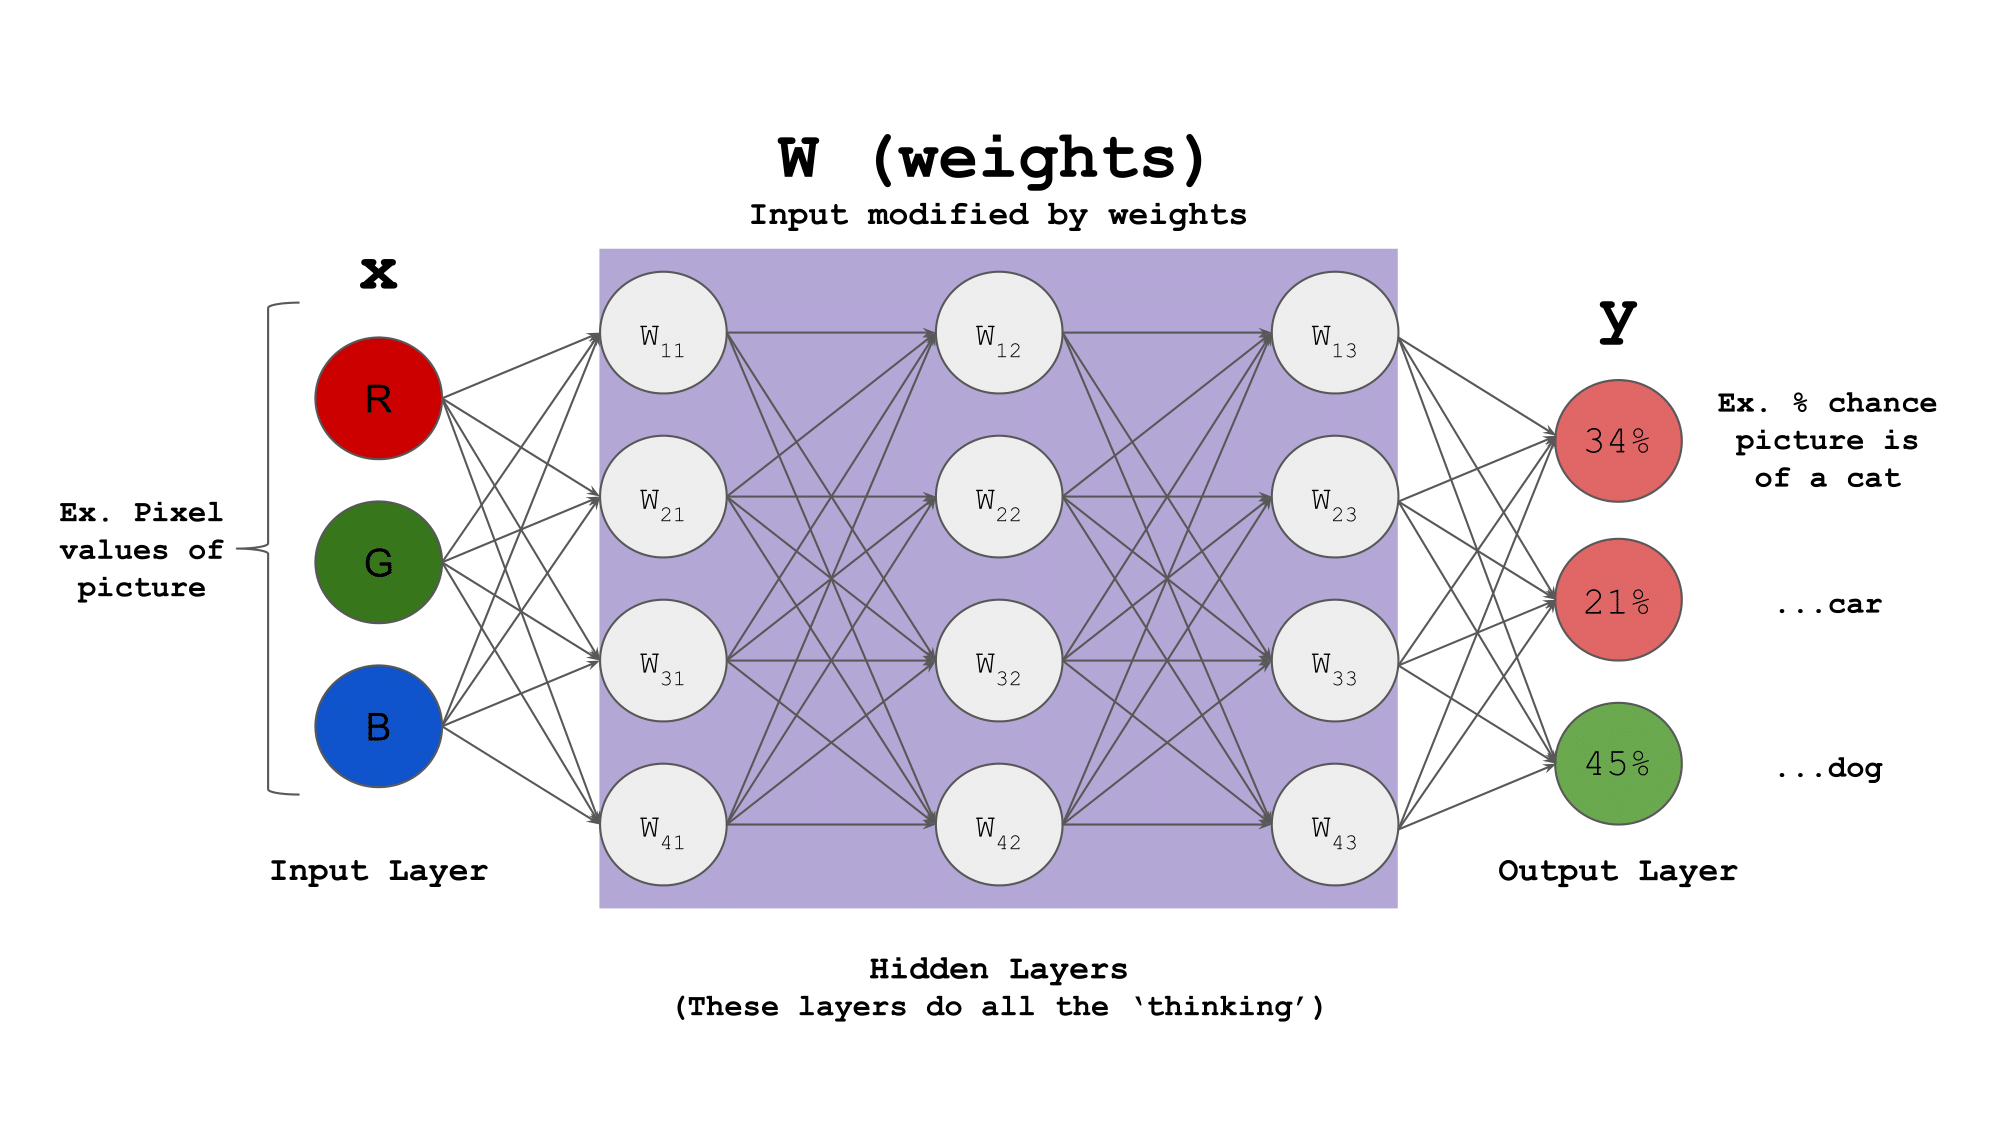
\includegraphics[width=1.35\linewidth]{ann}
\vspace{-1.3cm}
\caption*{A generic diagram of an ANN.}
\end{figure}

The input layer is the raw input, in our case its the preprocessed image (which
we flatten from a 2D matrix to a 1D vector). Each entry of this vector corresponds to a single pixel.

The hidden layers are where
abstraction takes place, for the most part. What goes on in these layers is, big surprise, hidden to the programmer. Its exact contents constantly update as the network learns. The large number of connections between each layer give neural networks great leeway in the kind of models they can produce. In our case, we'll only be using one hidden layer as Pong is relatively simple.

Finally, the output layer returns some percentage of confidence in a particular answer. In our case the paddle can only move up or down, so we only need 1 output: the confidence in moving down. Since there are only two options the confidence in moving up is just:
$$\textrm{up\%}=1-\textrm{ down\%}$$
Note that the layers in neural networks can be of any size. A common arrangement is having inputs of higher dimension that want to be \textit{distilled}, so to speak, into lower dimensional output (e.g. an image to some text labeling the image). In this case, the layers get gradually smaller and smaller until they reach the desired output size. This forces the network to have relatively low level abstractions at the bottom like edges and shadows, and higher level ones on top like appendages or facial features. The choice of these \textit{hyperparameters} predetermine the complexity of the network before training even begins.

Another important feature of a neural network are the non-linear activation functions that occur after each layer. These are analogous to the firing potentials in real neurons. If the weights in a neuron don't meet some threshold (defined by the activation function) then they're input is not sent to the next neuron (or in this case is severely weakened). This introduces a sort of discreteness to each layer and is what keeps our network, both in our brains and computers, from melding together into one continuous and uninteresting state.

And on top of all of this, notice that each line in the diagram represents a weight. All of these weights can be collected into a single matrix. It is in this way that we can convert the more intuitive model of neurons connecting to each other to the more practical model of matrix multiplication.

Putting these 3 facts together, we can represent our simple neural network via the following equation:
$$y = \mathrm{activate}(W\mathbf x)$$
\textit{Here $\mathrm{activate}$ is the activation function, $\mathbf x$ is our input of pixels, $W$ is the weight matrix of our hidden layer (which we have yet to adjust via training), and $y$ is our output (i.e. the percent confidence in moving down vs. up)}

\subsection{Training the Network}
We constructed our network above, and gave it the necessary room to represent all sorts of interesting abstractions. But until we train it, that capacity is wasted. We do this by using an algorithm called gradient descent. The goal of gradient descent is to minimize some function, in our case it is to minimize the punishment the network receives (or equivalently maximize the reward). Imagine if our input was only 1 dimensional, gradient descent would look something like this:

\begin{figure}[H]
\centering
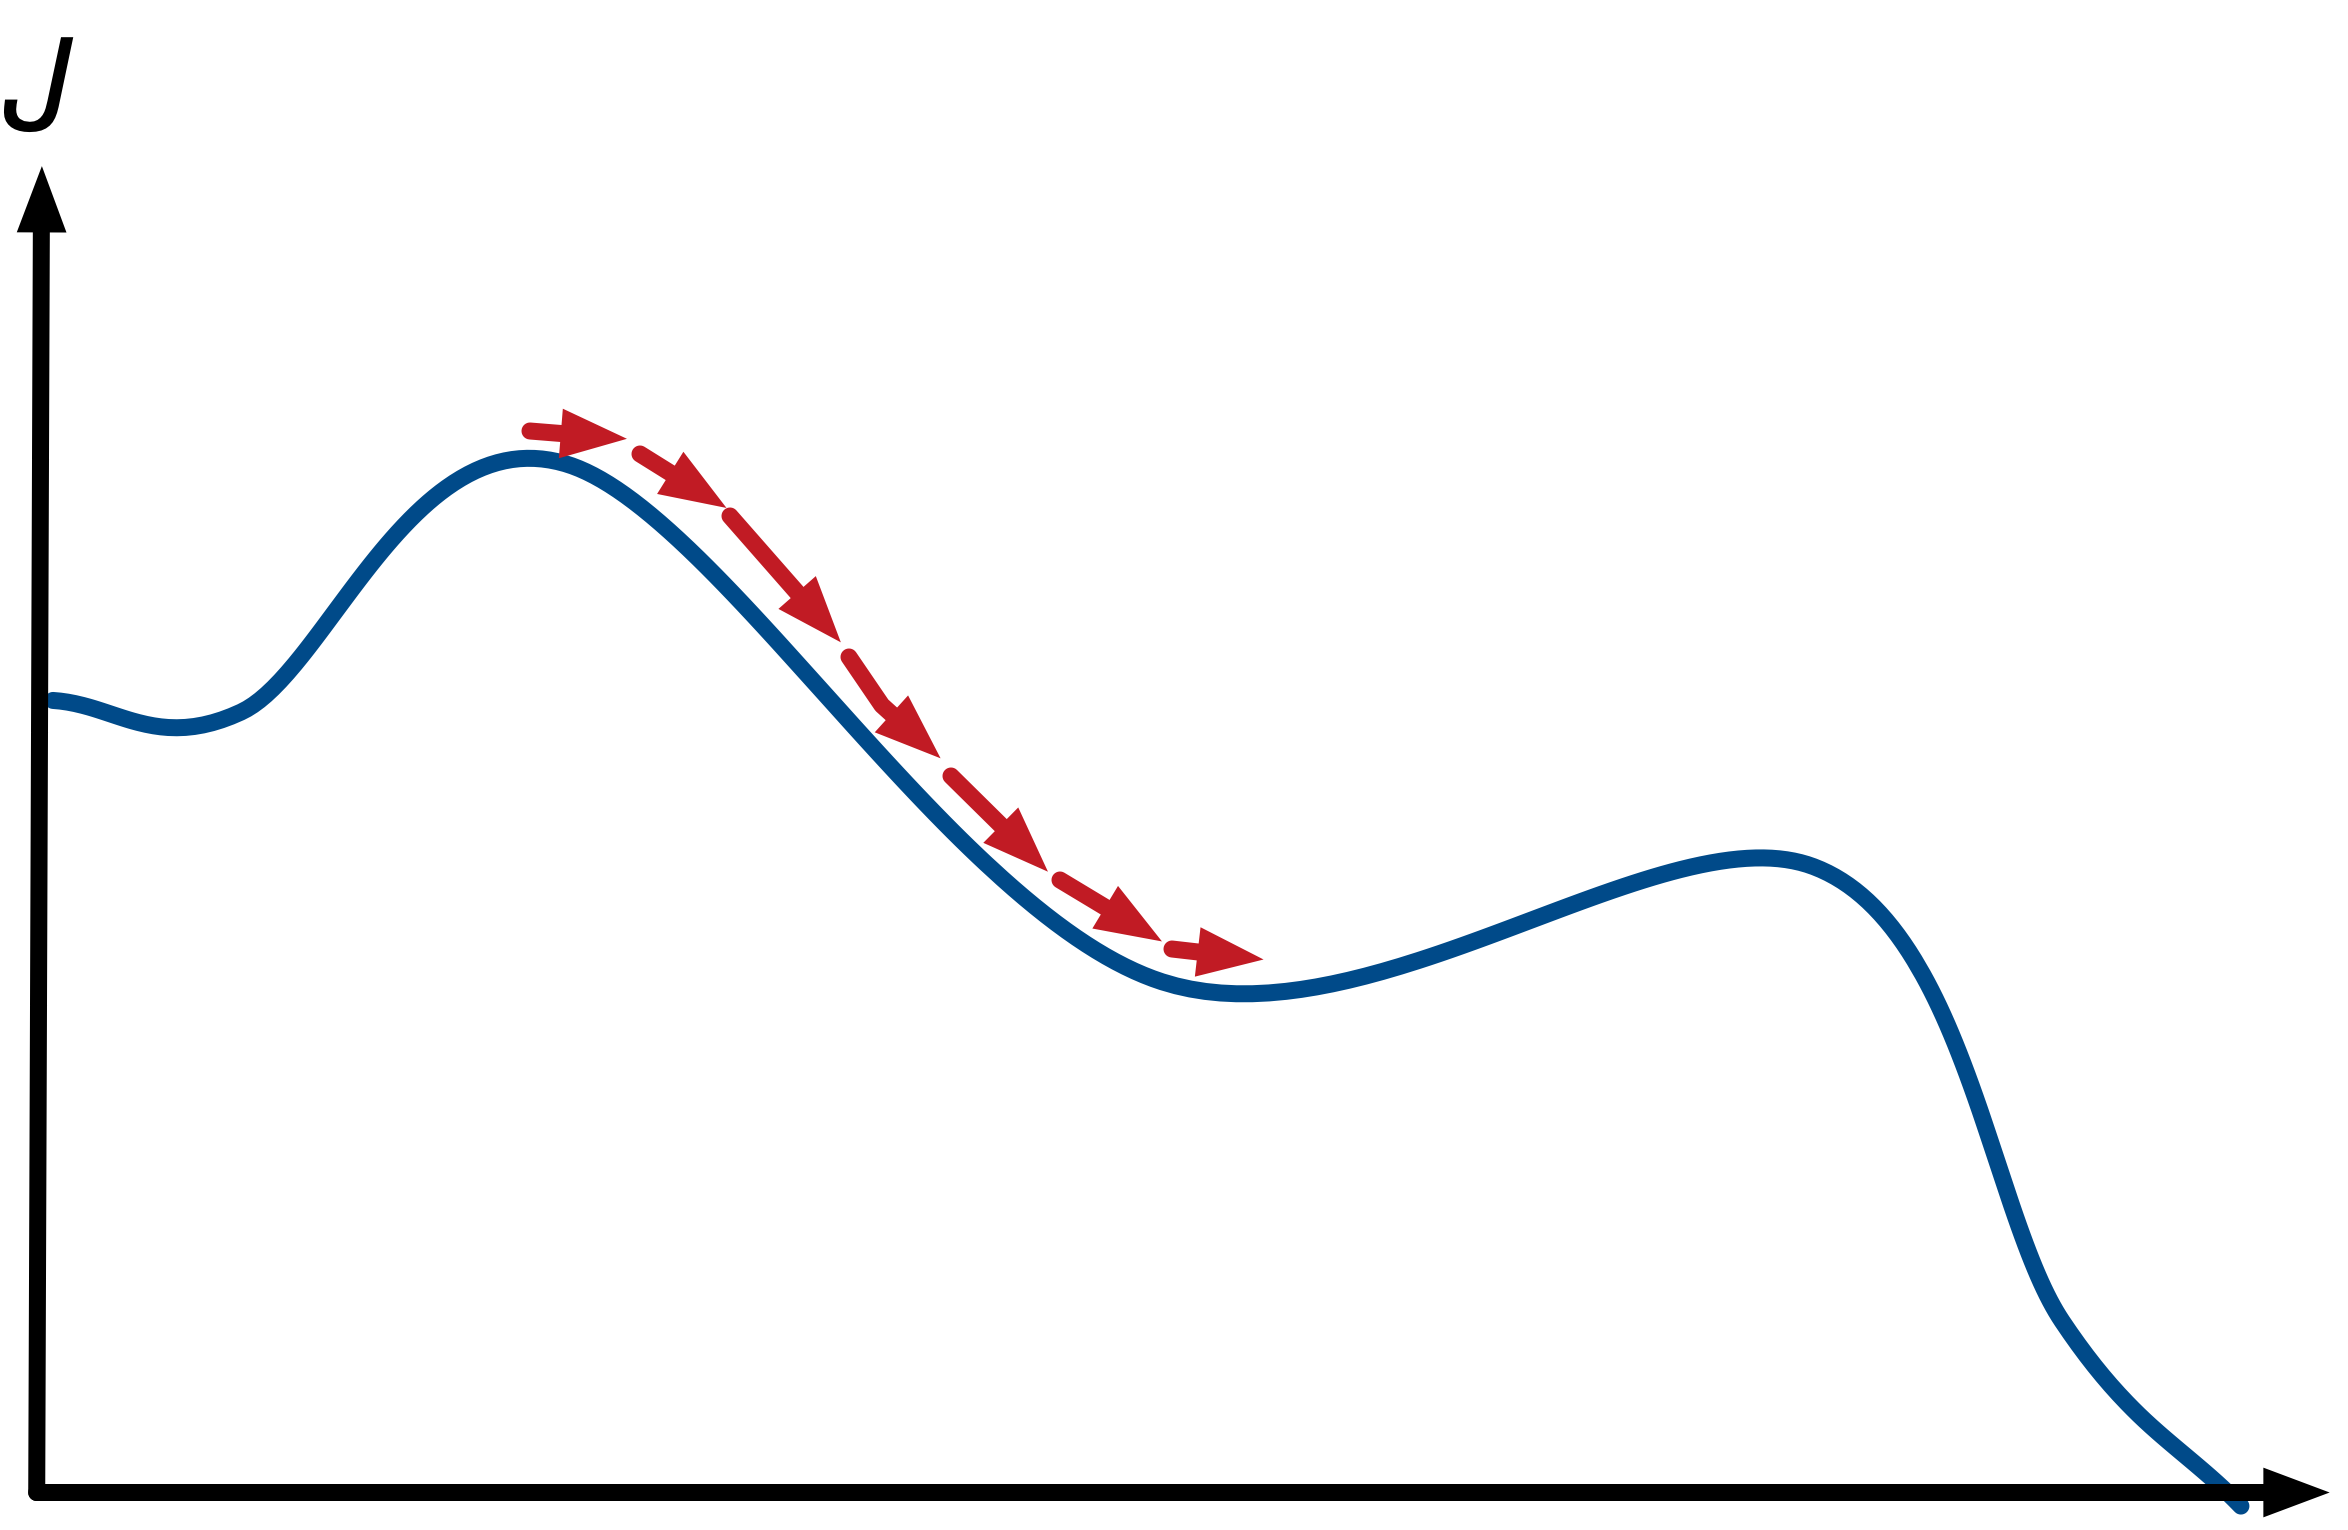
\includegraphics[width=.5\linewidth]{2d}
\caption*{Gradient descent in 2 dimensions.}
\end{figure}

The gist of it is that we take derivatives of the reward function with respect to each weight in the network and slightly nudge the weight in the direction that would minimize the punishment. Doing this over and over lets the punishment fall lower and lower, making our network more effective at playing Pong (assuming we rewarded/punished our network appropriately when it succeeded/failed)

Notice that even though there is a lower point further to the right of the graph, it is blocked by a hump. Gradient descent is what's called a greedy algorithm, and so only cares for what's immediately in front of it. This limitation is inherent in almost any optimization algorithm and can't really be avoided. Despite this, we can still make quite good neural nets in practice.

That was only a 2 dimensional representation of the scenario. Since our actual input has a dimension in the hundreds, the gradient descent takes place in a super high dimensional hyperspace. Since we can't visualize such a space, we'll have to settle for this 3D representation instead:

\begin{figure}[h]
\centering
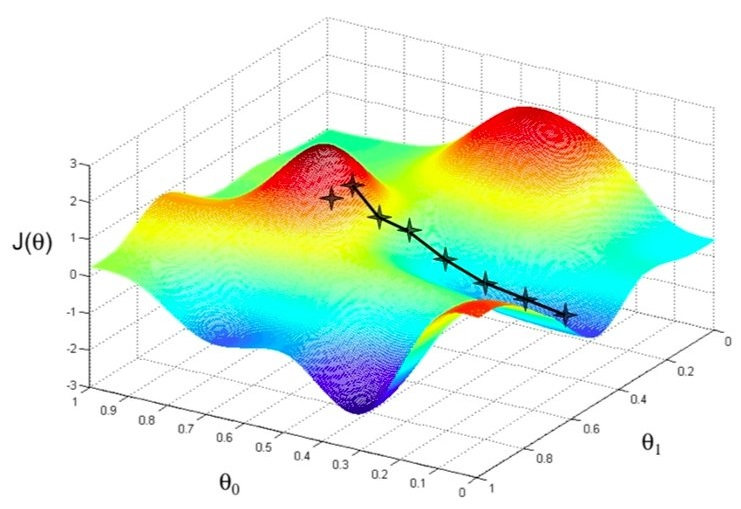
\includegraphics[width=.7\linewidth]{3d}
\caption*{Gradient descent in 3 dimensions.}
\end{figure}

\section{Evolving Views on Thought}
\subsection{Goalposts of Classical AI}
The proliferation of machine learning algorithms like the one we constructed above has had, and will surely continue to have, a profound impact on our contemporary society. An important facet of this impact is how people and the public view, not just artificial intelligence, but intelligence in general.

To be sure, ever since the first digital computers came into use and more and more challenging problems brought into their domain, we have always been dazzled at their sheer effectiveness. But the task of creating a thinking machine has always eluded us. Whenever a goal thought to have required thought was set for a machine, computer scientists have always stepped up to the challenge and delivered. But due to the nature of programming, by solving this, at first, intellectual seeming task, the programmers necessarily uncover that the problem can actually be solved via an understandable and mindless step of instructions. If it wasn't how else could one program a machine to do it? This leads those who set the goalpost of machine borne thought to retract their test with a ``that doesn't count, it isn't real thinking."

\subsection{Machine Learning is Different (maybe)}
And this is a fair point. It could hardly be said that a chess AI thinks in a way nearly as complex as a human being does, despite chess being once thought to be a test of true original thinking. But this new wave of AI, I posit, is different. Unlike past attempts at `hard-coded' AI, these new algorithms can not just learn on their own, but in a manner too complex for us to manually recreate. No person could go through a neural network and discern its function from the mess of numbers they would find, especially with deeper ANNs. Indeed, we know that the network is probably using some sort of process of \textit{abstraction} to \textit{distill} the information from the input into the output, but we can't put that process into concrete terms. This is very much analogous to our understanding of the brain. We can study the individual neurons and even networks of neurons in our brains via a variety of imaging techniques and we know that our brains must process information via some sort of abstraction, but saying much more is quite difficult.

Moving even further, at what point would one be willing to accept that there is no difference between a sufficiently advanced artificial neural network and that of a human, if such a point exists? Despite all the complexity of an ANN, it still is just a numerical algorithm. Yet, isn't that what a brain is?

In any case, the question of what this means in reality is one for another time. What \textit{we} are concerned with is the public's \textit{perception} of this new wave of AI, and the similarities between ANNs and our own biological neural networks may form an intuitive association between the two. Indeed the name the \textit{neural network} alludes to the eponymic neurons in our own brains and thus only strengthen this intuition.

\subsection{The Fundamental Question}
That said, it is important to distinguish the complexity of our own brains to that of ANNs like the one detailed in this paper. While more complex ANNs may exist in the future, the sheer complexity of the human brain is not comparable to a couple of matrix multiplications and non linear activation functions. And in a similar vain, learning in humans is certainly more than just a couple (thousand) passes of gradient descent, this much is clear. But is it comparable to millions? Billions? As these technologies, methods, and mathematics encroach closer and closer to the capabilities of man, the public will soon have no choice to shy away from the fundamental question of intelligence: ``What is thought?"

Certainly a machine couldn't think, right? Some pile of equations running through some silicon. Yet science has shown us time and time again that we too are quite similar: a pile of chemical laws running through some flesh. And when the capability of machines reaches or, eventually, eclipses that of man (by whatever measure you prefer) the question will no longer be one of ``does it think or not." Faced with an increasingly mechanical view of thought, the question becomes: do we include those machines as beings who think, or do we abandon the idealized notion of thought we've held for all these millennia?

\begin{thebibliography}{999}
\bibitem{dm}
  Mnih, Volodymyr, et at.\\
  \emph{Asynchronous Methods for Deep Reinforcement Learning}, Google DeepMind, 2016
\bibitem{dm}
  Karpathy, Andrej\\
  \emph{Deep Reinforcement Learning: Pong from Pixels}, Google DeepMind, 2016
\end{thebibliography}
\end{document}
